\documentclass[10pt,a4paper]{article}
\usepackage{graphicx}

\usepackage{slashbox}			% Diagonale Tabellenstriche
\usepackage{wrapfig}			% Grafiken in fließtexte einfügen
\usepackage{multirow} 			% Tabellen mit multiplen Spalten und Zeilen
\usepackage{enumerate}			% Nummerierte Listen erstellen
\usepackage{colortbl}	

\begin{document}
%\chapter{MOT Einführung}
\section{Definition des \textit{MOT}}
	\textit{MOT} (\textit{Multiple Object Tracking}) ist ein sequenzieller Prozess, bei dem Messungen genutzt werden, um die Anzahl und den dynamischen Zustand (Position und Geschwindigkeit) der Objekte zu bestimmen. Dabei basiert dieser Vorgang auf der Detektion. Abbildung \ref{fig: Zusammenhang zwischen Detektion und MOT} zeigt diesen Zusammenhang. Der Sensor liefert dem Detektor Daten, die zur Erstellung von Messungen verwendet werden. Danach wird ein \textit{MOT}-Algorithmus genutzt, um A-posteriori-Wahrscheinlichkeitsdichten für die Objektzustände zu ermitteln. Als Sensor dient beispielsweise eine Kamera, die dem Detektor Bilddaten übermittelt. Messungen können dann in Form von Punkten (Koordinaten in Pixelbereich), Bounding Boxen, etc., dem Algorithmus übergeben werden.
	\begin{figure}[h]
		\centering
		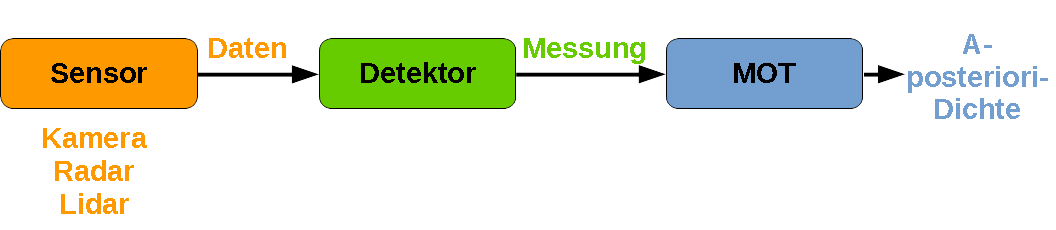
\includegraphics[width=0.7\linewidth]{./Pictures_report/Zusammenhang zwischen Detektion und MOT.png}
		\caption{Zusammenhang zwischen Detektion und \textit{MOT}}
		\label{fig: Zusammenhang zwischen Detektion und MOT}
	\end{figure}
\section{Herausforderungen in \textit{MOT}}
	Abbildung\ref{fig: Sichtfeld beim MOT} zeigt die grundlegende Problematik beim \textit{MOT}. Die Anzahl der zu erfassenden Objekte ist in der Ausgangssituation unbekannt, genauso wie deren Zustände. Der Grund dafür ist, dass hier dynamische Objekte vorliegen, die in Bewegung sind. Dadurch besteht die Möglichkeit, dass Objekte das Sichtfeld (engl. Field of View) sowohl betreten (Object-Birth) als auch verlassen (Object-Death) können. Ein weiteres Problem stellt das gegenseitige Verdecken der Objekte dar. Ebenfalls von sehr großer Bedeutung ist das unvollkommene Verhalten von Sensoren und Detektoren, weshalb man keine perfekten Messdaten erwarten darf. Aufgrund dessen ist man sehr anfällig für zwei Arten von Fehlern, Fehl- bzw. Missdetektion und Falschdetektion.
	\begin{figure}[h]
		\centering
		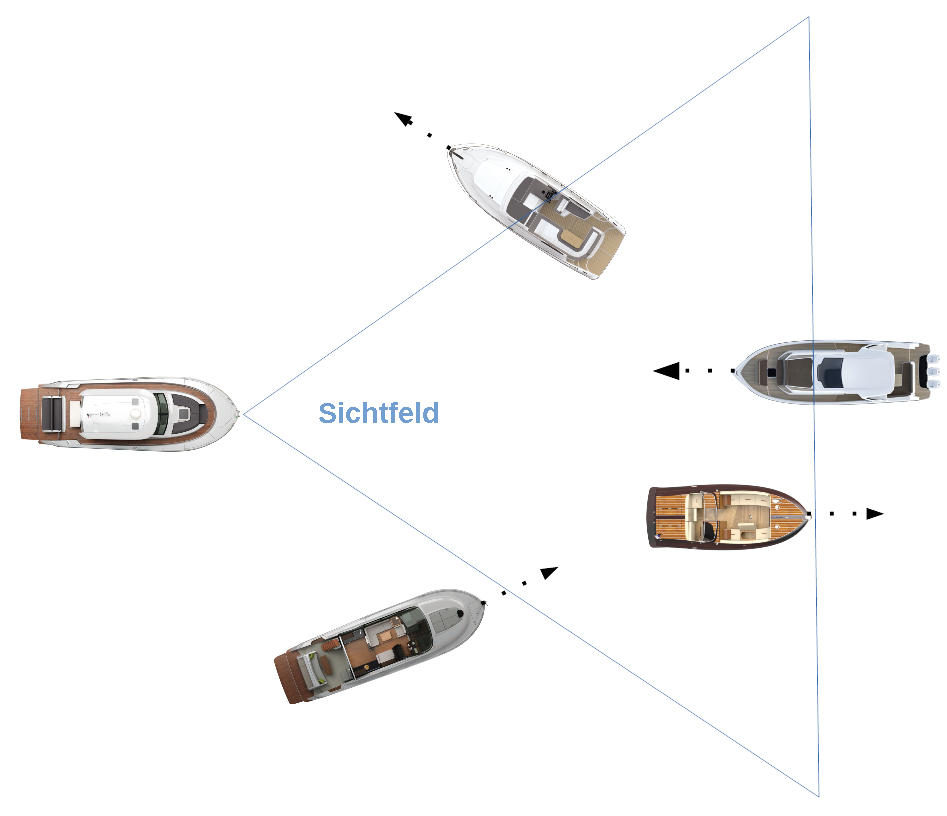
\includegraphics[width=0.5\linewidth]{./Pictures_report/Sichtfeld beim MOT.png}
		\caption{Sichtfeld beim \textit{MOT}}
		\label{fig: Sichtfeld beim MOT}
	\end{figure}
	\newline
	Bei einer Fehldetektion werden tatsächlich vorkommende Objekte im Sichtfeld nicht entdeckt. Gründe hierfür können Umweltbedingungen sein, welche die Sichtverhältnisse verschlechtern, zum Bsp. Nebel, Lichtverhältnisse, oder die Eigenschaften des Objekts selbst (Größe, Form, etc.). Im Falle einer Falschdetektion kommt es zu einer Detektion, die nicht aus einem Objekt resultiert. Dies wird auch als \textit{Clutter} bezeichnet. Auch hier sind Umweltbedingungen ein Faktor für dieses Fehlverhalten, aber auch das Sensorrauschen spielt eine Rolle. Bei der Modellierung muss das unvollkommene Verhalten von Sensor und Detektor immer berücksichtigt werden, um fatale Szenarien möglichst zu vermeiden.
	\newline
	Ein weiteres Problem stellt die Datenassoziation dar. Hierbei handelt es sich um einen Prozess, bei dem Messpunkte mit einem bereits bekannten \textit{Track} (geschätzte Trajektorie eines Objekts) assoziiert werden. Dies ist allerdings schwierig, da eine Datenassoziation nicht immer als bekannt angenommen werden kann. Abbildung \ref{fig: Vergleich bei bekannter und unbekannter Datenassoziation} veranschaulicht das Problem. Ist die Datenassoziation bekannt, so ist es recht einfach herauszufinden welche Messpunkte von den entsprechenden Objekten abstammen oder aus \textit{Clutter} resultieren. Bei einer unbekannten Datenassoziation sieht das anders aus. Man hat keinerlei Informationen darüber welche Detektionen zu den Objekten gehören, die schon vorher detektiert wurden. Genauso wenig weiß man, ob ein Messpunkt zu einem Objekt gehört, welches erst neulich das Sichtfeld betreten hat oder ob es sich einfach um \textit{Clutter} handelt. Dies führt zu einer hohen Anzahl an Assoziationsmöglichkeiten bzw. Hypothesen, die mit steigender Objektzahl sehr schnell zu nimmt. Der Umgang mit diesen Unsicherheiten wird zunehmend durch Sensorauschen, geringe Detektionsraten und Objekte mit sehr kleinem Abstand zueinander erschwert.
	\begin{figure}[h]
		\centering
		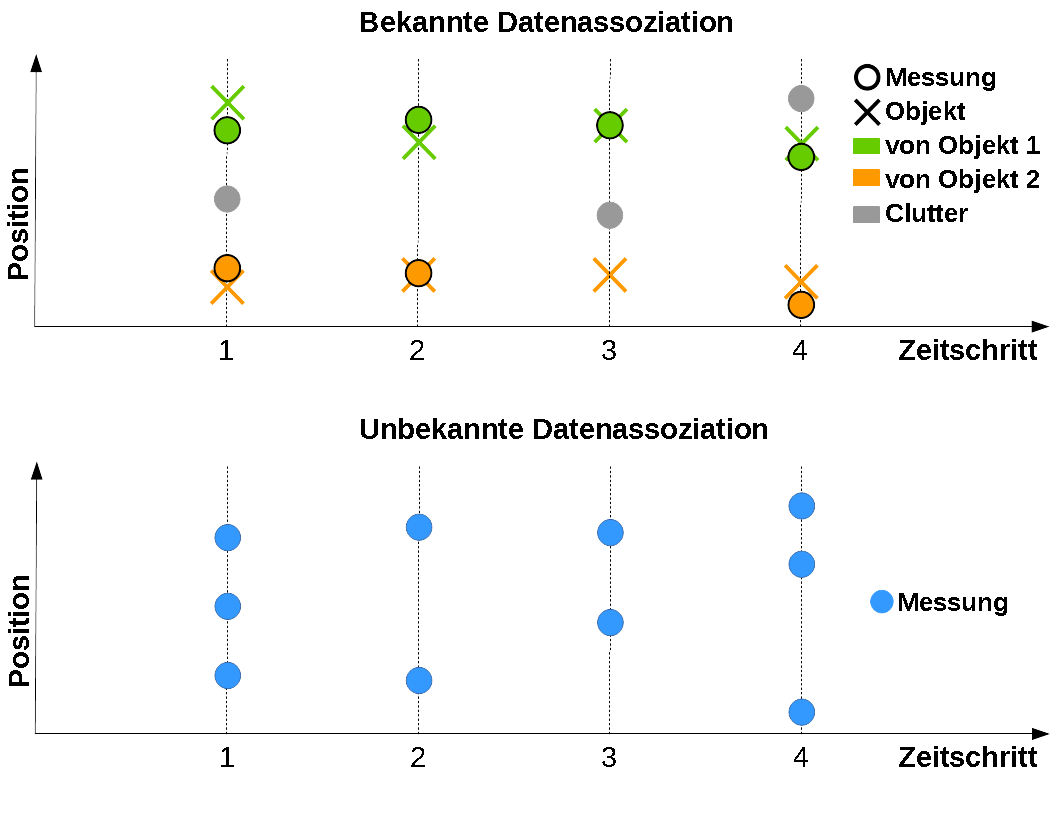
\includegraphics[width=0.5\linewidth]{./Pictures_report/Vergleich bei bekannter und unbekannter Datenassoziation.png}
		\caption{Vergleich bei bekannter und unbekannter Datenassoziation}
		\label{fig: Vergleich bei bekannter und unbekannter Datenassoziation}
	\end{figure}
	\newline
	Um die Anzahl an Hypothesen und den Rechenaufwand beim \textit{Tracking} möglichst gering zu halten gibt es zwei grundlegende Vorgehensweisen, \textit{Pruning} und \textit{Merging}. Beim \textit{Pruning} werden Assoziationsmöglichkeiten entfernt, die niedrig gewichtet wurden und somit unwahrscheinlich sind. Vereinigt man mehrere Hypothesen zu einer reduzierten Anzahl miteinander, handelt es sich um \textit{Merging}. Hierbei können Hypothesen, die sich ähnlich sind, zusammengefasst werden. Beide Vorgehensweisen können einzeln für sich oder miteinander kombiniert verwenden. Eine weitere Möglichkeit die Menge an Hypothesen zu verringern ist das sogenannte \textit{Gating} welches dem \textit{Pruning} ähnelt. Allerdings arbeitet man beim \textit{Gating} nicht mit Gewichtung, sondern mit Schranken (\textit{Gates}), welche die prädizierten Messpunkte umhüllen (Abbildung \ref{fig: Gating}). Aktuelle Messungen innerhalb einer Schranke können mit dem entsprechendem, vorherbestimmtem Wert assoziiert werden, während man Messpunkte außerhalb vernachlässigt.
	\begin{figure}[h]
		\centering
		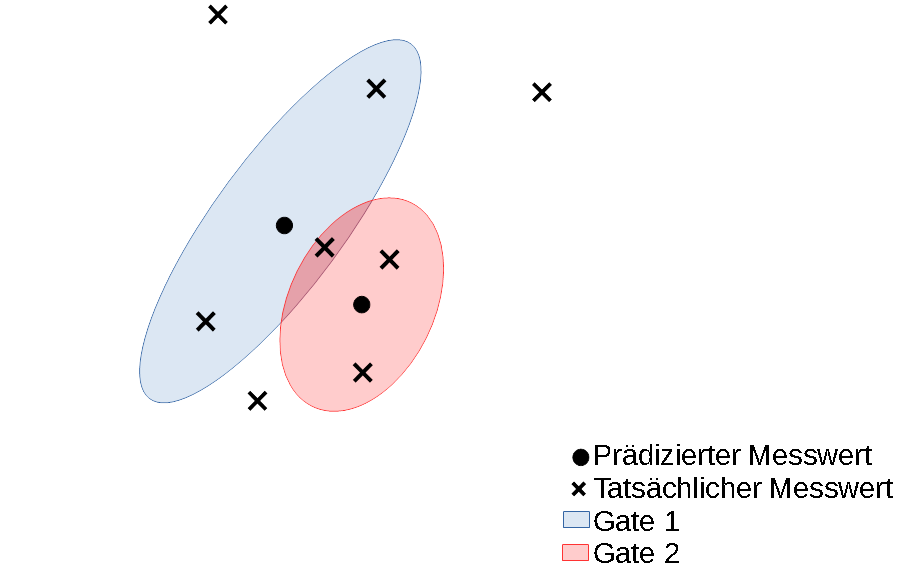
\includegraphics[width=0.50\linewidth]{./Pictures_report/Gating.png}
		\caption{Gating zum Zeitpunkt k}
		\label{fig: Gating}
	\end{figure}
\section{Notationen}
	Abschließend zu diesem Kapitel werden in Tabelle \ref{tab: Notationen} Notationen aufgelistet, die man in dieser Arbeit nutzt.
	\begin{table}[h]
		\centering
		\begin{tabular}{|l|l|}
			\hline
			$[.]_k$					&Index für den Zeitschritt\\ \hline
			$[.]_{1:k}$				&Index für einen Zeitabschnitt von 1 bis k\\ \hline
			$[.]_{k|k-1}$			&Index für prädizierten Wert\\ \hline
			$[.]_{k|k}$				&Index für korrigierten Wert\\ \hline
			$\underline{[.]}$		&klein Buchstaben mit Unterstrich sind Vektoren\\ \hline
			$\hat{[.]},\tilde{[.]}$	&Buchstaben mit Dach oder Tilde sind geschätzte Werte\\ \hline
			$\textbf{A}$			&dick gedruckte Buchstaben für Matrizen\\ \hline
			
	\end{tabular}
		\caption{Notationen}
		\label{tab: Notationen}
	\end{table}

\end{document}